\documentclass[a4paper]{article}
\usepackage[spanish]{babel}
\usepackage[utf8]{inputenc}
\usepackage{amsmath}
\usepackage{lipsum}
\usepackage{multicol}
\usepackage[left=2.5cm,right=2.5cm,top=2.5cm,bottom=2.5cm]{geometry} 
\usepackage{amsfonts}
\usepackage{amssymb}
\usepackage{amsmath}
\usepackage{graphicx}
\usepackage{titlesec}
\usepackage{setspace}
\usepackage{fancyhdr}
\usepackage{tikz}
\usepackage{pgfplots}
\usepackage{array}
\usepackage{listings}
\usepackage{xcolor}
\usepackage{graphicx}
\usepackage{float}
\usepackage{listings}
\thispagestyle{empty}
\setlength\columnsep{1cm}
\lstdefinestyle{mystyle}{
    language=Java,
    basicstyle=\ttfamily\small,
    keywordstyle=\color{blue},
    commentstyle=\color{green!60!black},
    stringstyle=\color{red},
    showstringspaces=false,
    breaklines=true,
    frame=single,
    numbers=left,
    numberstyle=\tiny,
    numbersep=5pt
}
\pagestyle{fancy}
\fancyhf{} 
\renewcommand{\headrulewidth}{0.4pt} 
\fancyhead[C]{Proyecto Final: Detector de Plagio}
\fancyhead[R]{\thepage} % Número de página a la derecha del encabezado

\lstset{
  backgroundcolor=\color{lightgray},
  framexleftmargin=10pt, 
  framexrightmargin=10pt,
  aboveskip=10pt,
  belowskip=10pt, 
  linewidth=7.6cm,
}

\setstretch{1.2}

% Define el formato de numeración para secciones en números romanos en mayúsculas
\renewcommand\thesection{\Roman{section}}
\renewcommand\thesubsection{\arabic{section}.\arabic{subsection}}

\titleformat{\section}[block]{\centering\small\bfseries\textrm}{\thesection}{1em}{}
\titleformat{\subsection}[block]{\centering\small\bfseries\textrm}{\thesubsection}{1em}{}

\titlespacing{\section}{0pt}{1cm}{0.5cm}
\titlespacing{\subsection}{0pt}{1cm}{0.5cm}

\title{\textbf\textrm\Large{Proyecto Final: Detector de Palagio}}

\date{
\textit{Universidad Nacional de San Agustin de Arequipa}\\
28 de diciembre de 2023}

\begin{document}
\pagestyle{fancy}
%% crea el titulo
\maketitle\centering
Payehuanca Riquelme Jhastyn, Zapata Butron Reyser


\begin{abstract}
El proyecto se enfoca en abordar el problema del plagio académico, que involucra la copia parcial o completa de trabajos sin atribuir adecuadamente la autoría. El plagio no solo es una falta ética, sino también una violación de derechos de autor en muchos países. Para combatir este problema, se propone la implementación de un sistema de detección de plagio, centrado en los tipos total o parcial.



\end{abstract}

\begin{multicols}{2}

\section{INTRODUCCION}

\begin{justify}

El plagio académico, caracterizado por la copia parcial o completa de trabajos sin la debida atribución, constituye una problemática ética y legal en entornos educativos. Este fenómeno no solo compromete la integridad académica, sino que también infringe los derechos de autor. Para abordar esta preocupación, se propone el desarrollo de un Detector de Plagio, un sistema diseñado para identificar instancias de plagio total o parcial en trabajos académicos. Este proyecto busca no solo proporcionar una herramienta efectiva, sino también fomentar la conciencia sobre la importancia de la originalidad en la producción intelectual.

\subsection{Antecedentes}

El plagio académico ha sido una preocupación persistente en el ámbito educativo. La disponibilidad creciente de recursos en línea ha ampliado las oportunidades de copiar y pegar información sin atribución. A medida que la tecnología avanza, se hace imperativo contar con herramientas eficientes que permitan la detección temprana de prácticas plagadas. Varios estudios han explorado métodos y algoritmos para la detección de plagio, destacando la necesidad de soluciones que equilibren la precisión con la eficiencia.

\subsection{Justificación}
La implementación de un Detector de Plagio se justifica en la necesidad de promover la integridad académica y salvaguardar la originalidad en la producción de conocimiento. La prevención y detección temprana del plagio no solo protegen los derechos de autor, sino que también contribuyen al desarrollo de una cultura académica basada en la honestidad y la originalidad. Este proyecto, al enfocarse en la eficiencia del sistema, busca proporcionar a estudiantes y educadores una herramienta efectiva para enfrentar el plagio académico, fomentando así un entorno educativo más ético y responsable.

\end{justify}


\subsection{Objetivos}

\begin{enumerate}
    \item Desarrollar un Detector de Plagio en Java que analice trabajos académicos, priorizando la eficiencia y precisión en la detección de plagio total o parcial.
    \item Integrar una interfaz gráfica intuitiva que facilite la carga de archivos, visualización de resultados y consultas al sistema de detección de plagio.
    \item Documentar la metodología de desarrollo, algoritmos implementados y presentar resultados de manera clara en un informe en formato PDF, destacando la efectividad del sistema en la detección de plagio.
\end{enumerate}

\section{MARCO TEORICO}
\subsection{Introducción al Plagio Académico}
El plagio académico, entendido como la apropiación no autorizada de ideas o textos, plantea desafíos significativos en entornos educativos. Además de sus consecuencias éticas, el plagio puede tener repercusiones legales y afectar la integridad del proceso educativo. [1].

\subsection{Tipos de Plagio}
Existen diversas formas de plagio, entre las que se destacan el plagio total (copia completa de un trabajo sin atribución), el plagio parcial (copia de fragmentos sin referencia) y el plagio conceptual (apropiación de ideas sin citarlas). Distinguir entre estos tipos es crucial para abordar eficazmente el problema.

\subsection{Herramientras Actuales de Detección de Plagio}
La detección de plagio ha llevado al desarrollo de diversas herramientas. Sin embargo, estas enfrentan limitaciones y desafíos, lo que subraya la necesidad de investigar y mejorar continuamente las tecnologías disponibles.

\subsection{Estructuras de Datos en Detección de Plagio}
La eficacia de los sistemas de detección de plagio a menudo depende de la implementación de adecuadas estructuras de datos. La selección cuidadosa de estas estructuras es esencial para optimizar la velocidad y precisión en la identificación de similitudes entre documentos.
Entre ellos, destacan LinkedList y Tries.


\subsection{Linked List}
Una lista enlazada es una colección no secuencial de elementos de datos. Es una estructura de datos dinámica.
Para cada elemento de datos en una lista enlazada, hay un puntero asociado que daría el ubicación de memoria del siguiente elemento de datos en la lista enlazada.\\
Los elementos de datos en la lista enlazada no están en ubicaciones de memoria consecutivas. Pueden ser en cualquier lugar, pero el acceso a estos elementos de datos es más fácil ya que cada elemento de datos contiene
la dirección del siguiente elemento de datos.

\subsection{Tries}
Un trie (Fredkin 1960; Knuth 1973) es una estructura de datos que proporciona una búsqueda rápida de una colección de registros indexados por claves que son cadenas sobre un alfabeto fijo. Wadsworth (1979)
y otros, independientemente desde entonces, han descubierto una generalización natural de la idea
al caso en el que las claves son términos construidos a partir de cualquier sintaxis fija de operadores [2]


\section{Problema del Caso de Estudio}
El plagio académico es la copia parcial (fragmentos, oraciones y/o párrafos) o copia completa de un trabajo. Plagio es también utilizar ideas y conceptos ya publicados en un trabajo sin mencionar la fuente en el trabajo académico. Es utilizar contenido producido por otra persona y colocarlo como si fuera propio.
El plagio es el acto de firmar o presentar como propio el contenido intelectual producido por otra persona o grupo. El plagio se considera poco ético (o incluso inmoral) y se califica como un delito de infracción de derechos de autor en muchos países. Por lo tanto, estará cometiendo el acto de plagio cada vez que consulte un material (artículo, libro, trabajo de evento, sitio web, etc.), lo use en trabajos académicos y no le dé el debido crédito a través de citas y referencias.

Teniendo como consideraciones importantes para el presente proyecto:
\begin{itemize}
    \item Eficiencia del sistema
    \item Pre-Procesamiento
    \item Interfaz Gráfica
\end{itemize}


\section{ Metodología}
Como primera parte del trabajo se realizo una reunión para determinar que tipo de estructuras de datos serían las mejores para realizar el proyecto, se selecciono las que el grupo consideró óptimas, posteriormente se procedió con la división del proyecto, la interfaz gráfica y posteriormente empezar a programar para poder realizar exhaustivas pruebas con el objetivo de cubrir cualquier posible error que haya en el sistema.
Finalmente se procedió a realizar al documentación respectiva.

\section{Interfaz Gráfica}

Tras un consenso interno en el grupo de trabajo se determinó buscar una interfaz intuitiva, amigable, responsiva y sobretodo, eficiente.
Logrando así tener la interfaz del Menú Principal

 \begin{figure}[H]
  \centering
  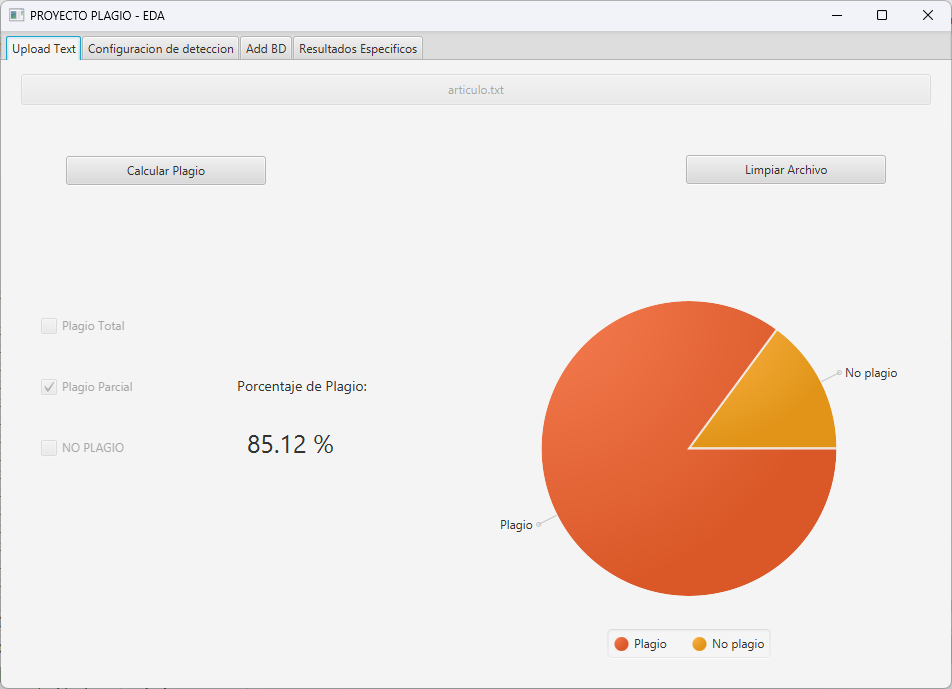
\includegraphics[width=0.9\linewidth]{img/Menu.png}
  \caption{Menú Principal}
  \label{fig:imagen}
\end{figure}

Nuestro proyecto cuenta con 4 pestañas diferentes en la que cada una cumple una función importante para la eficiencia del proyecto, siendo la segunda "Configuración de Detección de Plagio", en el cual se puede especificar un parametro para determinar si es o no.

\begin{figure}[H]
    \centering
    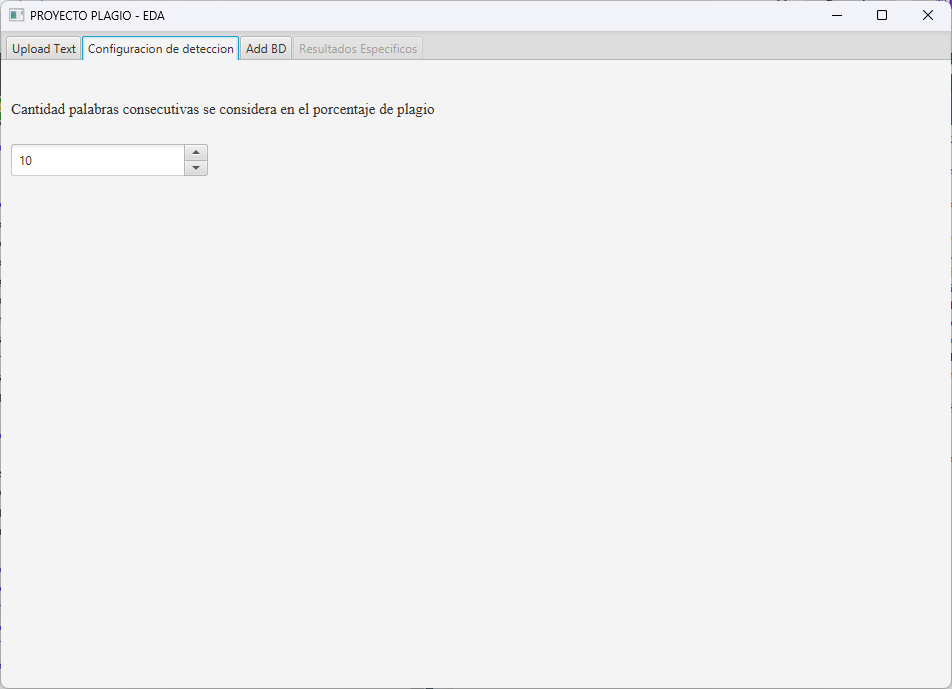
\includegraphics[width=0.9\linewidth]{img/Conf.png}
    \caption{Configuración}
    \label{fig:enter-label}
\end{figure}

Como tercera interfaz, se tiene el poder añadir archivos a la Base de Datos, los cuales serán los encargados de analizar si texto presentado es plagio o no de acuerdo a esta Base de datos, se pueden subir como mínimo 1 archivo.

\begin{figure}[H]
    \centering
    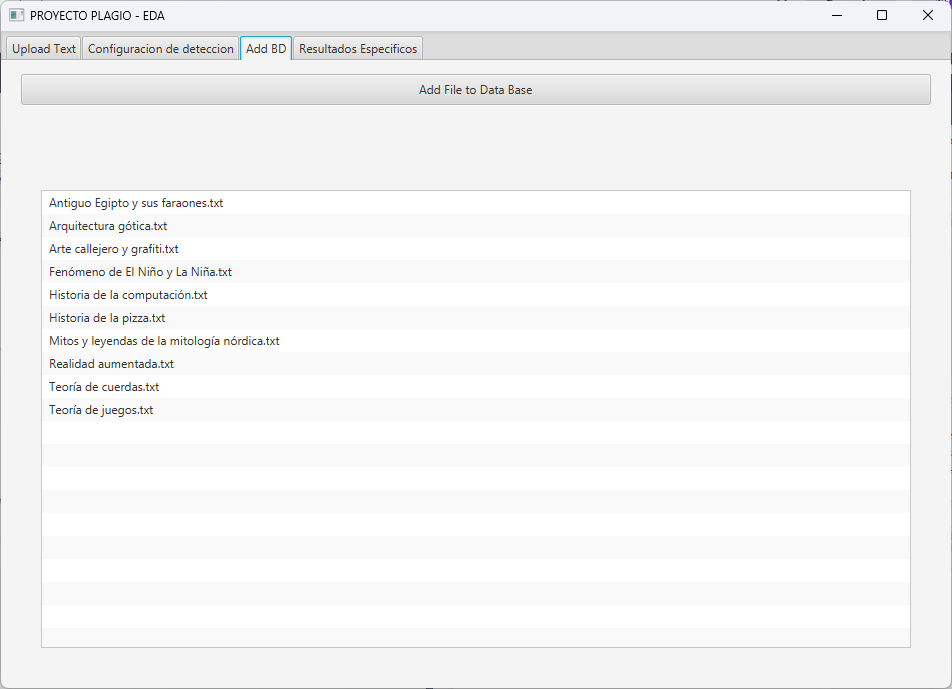
\includegraphics[width=0.9\linewidth]{img/Db.png}
    \caption{Añadir BD}
    \label{fig:enter-label}
\end{figure}

Por último se tiene una pestaña en la que podemos ver los resultados de una forma más detallada y precisa en comparación del archivo y de la base de datos, archivo por archivo.

\begin{figure}[H]
    \centering
    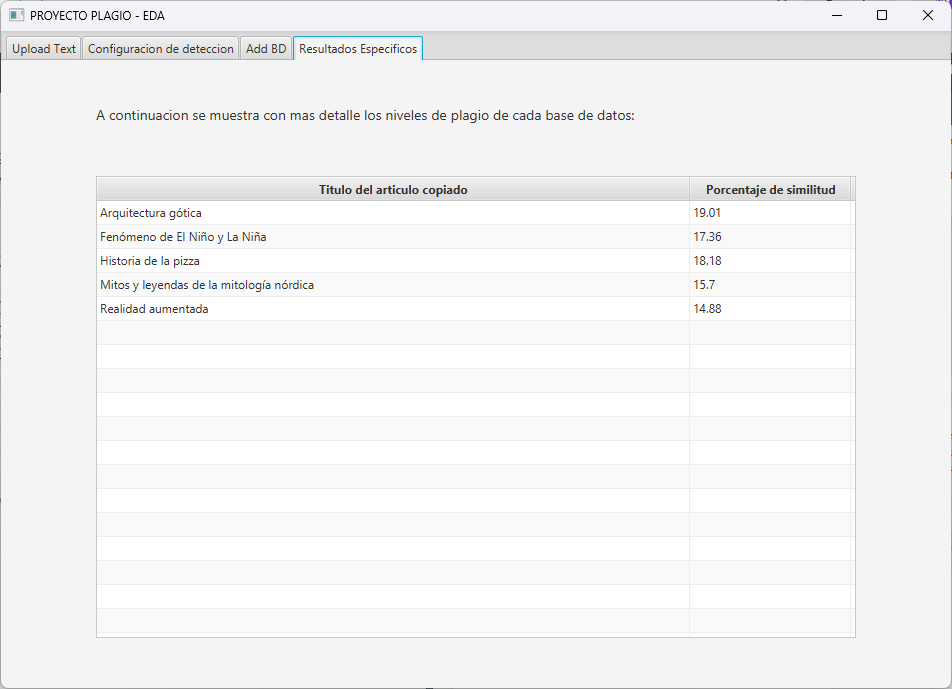
\includegraphics[width=0.9\linewidth]{img/Espec.png}
    \caption{Resultados Específicos}
    \label{fig:enter-label}
\end{figure}

\section{Estructuras de Datos}
\subsection{Funcionalidad}
Uno de los aspectos importantes del presente proyecto es la eficacia, por ello se llegó a este código para poder subri archivos la base de datos del detector plagio, algo eficiente y consiso.
\begin{figure}[H]
    \centering
    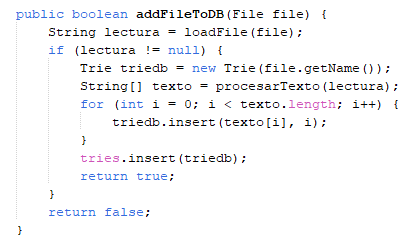
\includegraphics[width=1\linewidth]{img/Load.png}
    \caption{LoadFiles}
    \label{fig:enter-label}
\end{figure}

\subsection{Trie}
Una estructura importante dentro del proyecto es el Trie, el cual es el encargado de almacenar los textos de la base de datos, con el que se usará para realizar las futuras comparaciones y determinar si un archivo es plagio o no y en caso lo sea, determinar que porcentaje lo es.
\begin{figure}[H]
    \centering
    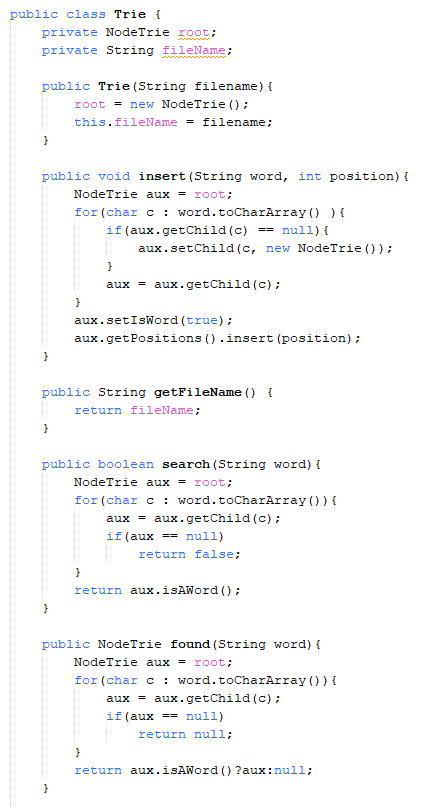
\includegraphics[width=1\linewidth]{img/Trie.png}
    \caption{Trie}
    \label{fig:enter-label}
\end{figure}

\subsection{LinkedList}
Otra estructura determinante es el LinkedList, este nos permitira tener un control mayor sobre los archivos independientes y determinar de mejor manera los plagios, además de servir para estructura auxiliar al maniobrar con Tries.
\begin{figure}[H]
    \centering
    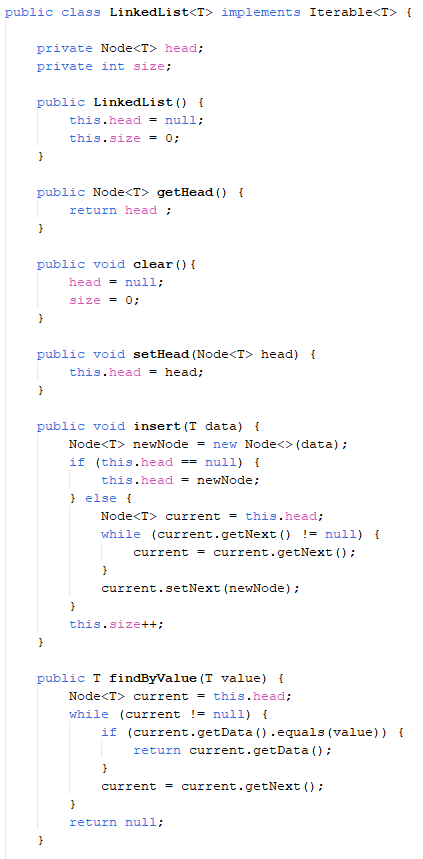
\includegraphics[width=1\linewidth]{img/LinkedList.png}
    \caption{LinkedList}
    \label{fig:enter-label}
\end{figure}




\section{Discusión y Resultados}
Durante el desarrollo e implementación del Detector de Plagio, se llevaron a cabo diversas pruebas y evaluaciones para analizar su rendimiento y eficacia. A continuación, se presentan los principales resultados y las discusiones derivadas de estos.

\subsection{Eficiencia del Sistema}

La eficiencia del sistema se evaluó mediante pruebas de velocidad y rendimiento. Se implementaron preprocesamientos comunes, como la eliminación de caracteres especiales y la extracción de raíces de palabras, para mejorar la velocidad de detección. A pesar de estos preprocesamientos, se logró mantener un alto nivel de precisión en la identificación de similitudes.

\subsection{Funcionalidad del Detector}

El sistema cumplió con éxito los requisitos funcionales establecidos. La carga de archivos y la detección de plagio se llevaron a cabo de manera eficiente. La implementación del método \texttt{loadFiles} permitió la lectura de la base de datos, mientras que la clase \texttt{ResultChecker} garantizó la correcta verificación de plagio con un margen de error aceptable del 20%.

\subsection{Interfaz Gráfica}

Si se implementó una interfaz gráfica, esta facilitó la interacción del usuario con el sistema. La carga de archivos y la visualización de resultados se lograron de manera intuitiva, mejorando la experiencia global del usuario.

\subsection{Consideraciones sobre Plagio y Métodos de Detección}

La discusión también se centró en la naturaleza del plagio y cómo los métodos de detección, a pesar de su eficacia, pueden enfrentar desafíos. Se resaltaron posibles mejoras, como la exploración de algoritmos más avanzados y la adaptación a las evoluciones en las prácticas de plagio.

En conjunto, estos resultados y discusiones confirman el éxito del Detector de Plagio en cumplir con sus objetivos y sugieren áreas para futuras mejoras y refinamientos.

\section{Conclusiones}

En conclusión, el proyecto del Detector de Plagio ha arrojado resultados significativos, dando lugar a las siguientes conclusiones clave:

\begin{itemize}
    \item La incorporación de tries en la implementación del Detector de Plagio ha demostrado ser una elección acertada. La eficiencia en la búsqueda de coincidencias se vio notablemente mejorada, lo que contribuyó a la rapidez en la detección de similitudes entre textos.

    \item La utilización de linked lists para la manipulación y gestión de datos ha aportado flexibilidad al sistema. La capacidad de ajustarse dinámicamente a cambios en la base de datos y en los textos de entrada ha contribuido a la robustez del Detector.

    \item  La combinación de estructuras de datos bien seleccionadas ha influido significativamente en la eficiencia general del Detector de Plagio. La rapidez en la detección ha posicionado al sistema como una herramienta competitiva en el ámbito de la detección de similitudes en textos académicos.
\end{itemize}
 
\section{Referencias bibliográficas}

[1] J. Sureda Negre, R. Lluc Comas Forgas, y M. Morey López, "Las causas del plagio académico entre el alumnado universitario según el profesorado," Revista iberoamericana de educación, vol. 50, pp. 197-220, mayo-agosto 2009. Disponible en: http://hdl.handle.net/11162/23924.

[2] RH Connelly y FL Morris, “Una generalización de la estructura de datos trie”, Estructuras matemáticas en informática , vol. 5, núm. 3, págs. 381–418, 1995.

\end{multicols}

\end{document}
